% \newpage
\section{Introduction}\label{Sec:introduction}
%%%%%%%%%%%%%%%%%%%%%%%%%%%%%%%%%%%%%%%%%%%%%%%%%%%%%%%%%%%%%%%%%%%%%%%%
\subsection*{Objectives}
In this paper 2 pieces of software are developed, one to detect the pose of a cylinder using and RGB-D camera and a second one to pick and place said cylinder in between 3 target locations. Additionally, once the first grasp is initiated, only bumper sensing will be used to keep track of the location of the cylinder object.

%%%%%%%%%%%%%%%%%%%%%%%%%%%%%%%%%%%%%%%%%%%%%%%%%%%%%%%%%%%%%%%%%%%%%%%%
\subsection*{Problem Setup}
The robot used for the pick and place task will be a Franka Emika Panda 7-DoF manipulator. The manipulator is set-up in the RViz environment shown in Figure \ref{fig:setup}.

The manipulator is directly facing a wall and the target cylinder to be picked, which is resting on the floor. The manipulator is also surrounded by 3 tables, which will serve as the target locations for the cylinder placement. 

Each table has a bumper sensor at its center that will indicate to the robot whether the table is occupied or not. One of the tables contains a box object that will have to be re-positioned to make space for the cylinder should it be moved to the same table.

The RGB-D camera will be placed as shown by the frame in Figure \ref{fig:setup}, pointing towards the wall and cylinder object.

\begin{figure}[h]
    \centering
    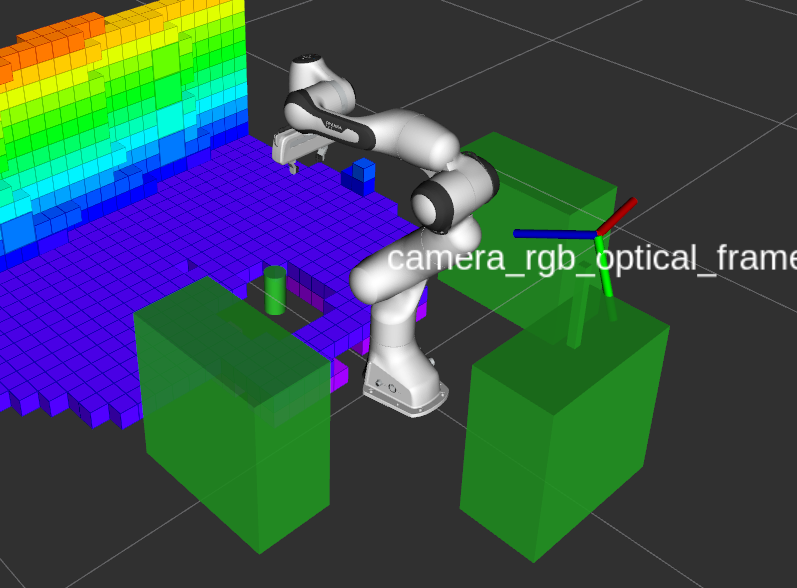
\includegraphics[width=8cm]{Images/Setup.png}
    \caption{RViz simulation environment setup. The voxel-grid indicates the floor and wall as perceived by the camera. MoveIt! collision objects are displayed in green.}
    \label{fig:setup}
\end{figure}

%%%%%%%%%%%%%%%%%%%%%%%%%%%%%%%%%%%%%%%%%%%%%%%%%%%%%%%%%%%%%%%%%%%%%%%%
\subsection*{Related Work}
The software used for cylinder detection makes use of the Random Sample Consensus (RANSAC) algorithm  \cite{RANSAC} to segment the RGB-D point cloud generated by the camera. Identifying (using RANSAC) the points of the point cloud that fit a cylindrical model, we are effectively removing the floor and wall from the point cloud. From those remaining points and the fitted model the cylinder's dimensions and pose can be ascertained. Both RANSAC and the point cloud management are implemented using the PCL library \cite{PCL}.

The robot path planning and control, the bumper sensors and the collision objects are implemented through the MoveIt! library \cite{moveit}.
